In fully-supervised settings regularization monotonically shrinks the learned value function. In bootstrapped settings regularization is recursively applied and so \textbf{the learned value function may counterintuitively increase as $\eta$ increases.}
\begin{center}
    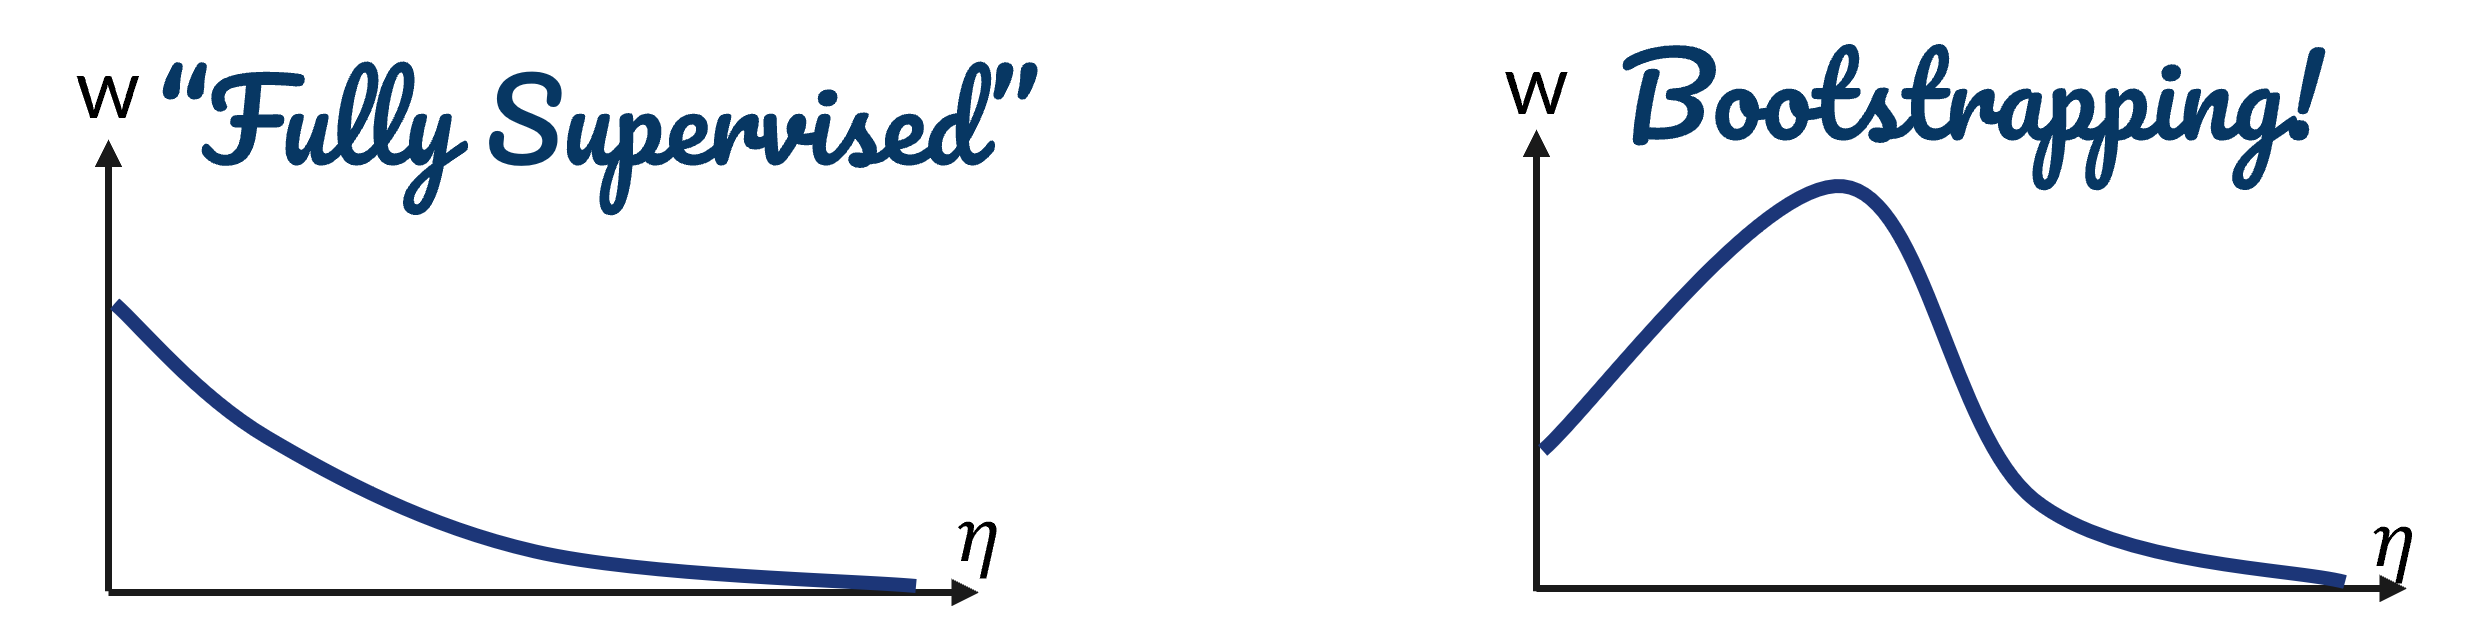
\includegraphics[scale=0.4]{parts/nonmonotonic/illus.png}
\end{center}
TD learning may diverge around specific--possibly multiple--values of $\eta$. In the first two plots below, the TD error increases sharply at specific amounts of regularization:
\begin{center}
    \hspace*{1in}
    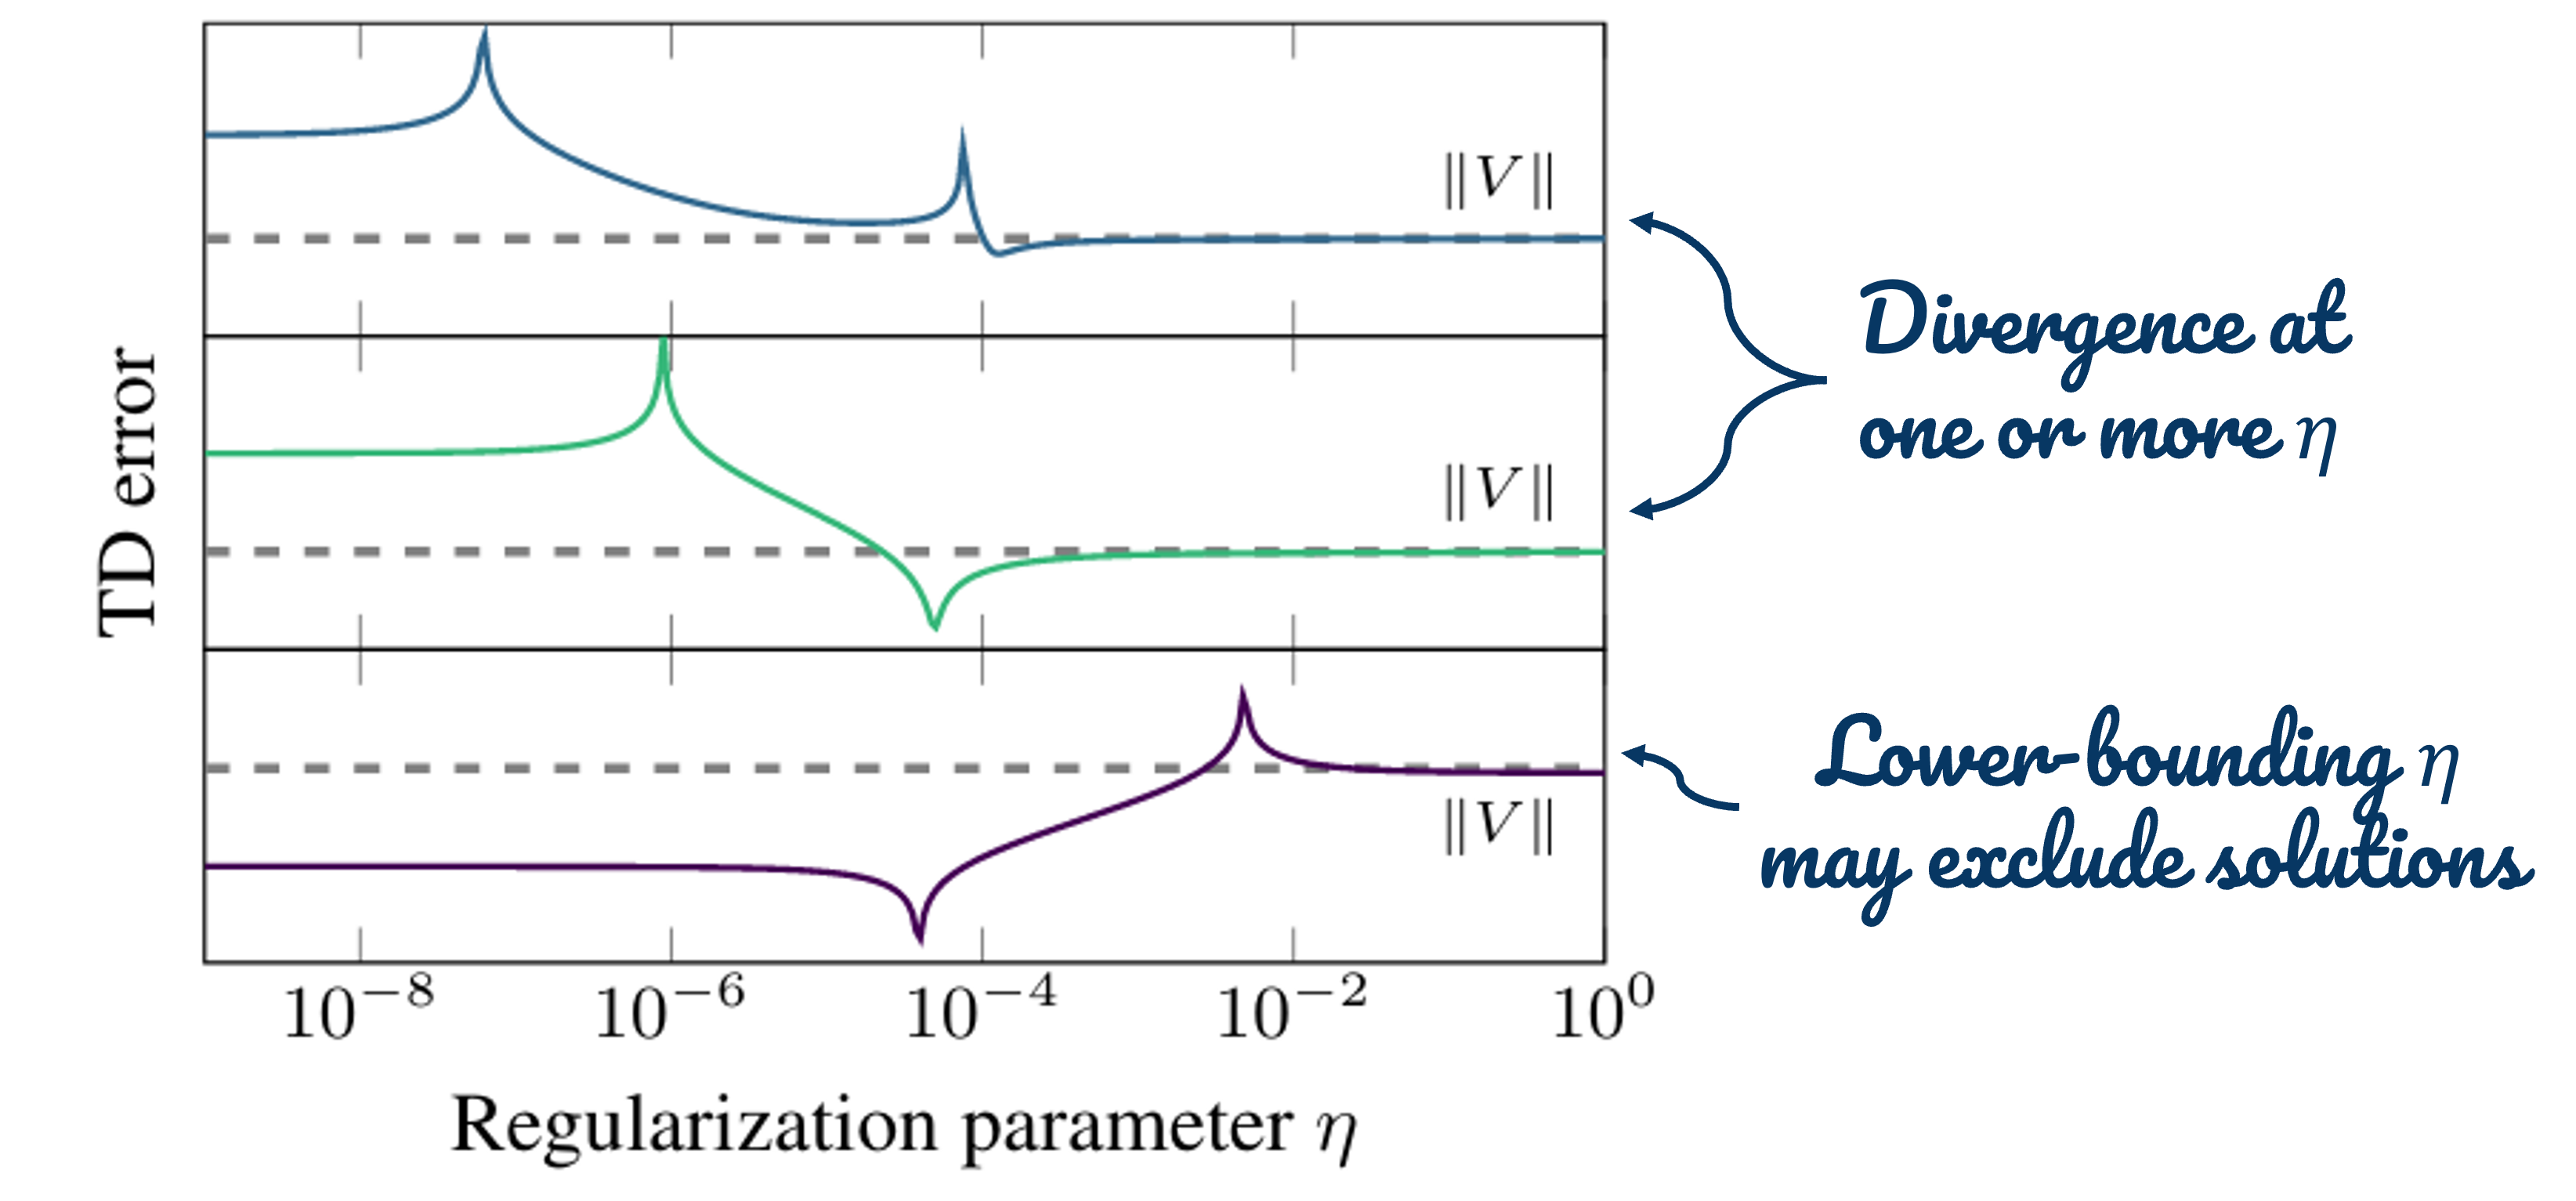
\includegraphics[scale=0.4]{parts/nonmonotonic/threeex.png}
\end{center}
In the literature a common fix for this problem is to assume that TD learning behaves ``almost-PSD'', and so will be well-behaved above some lower bound on $\eta$. In practice, this assumption is dangerous: it may restrict us to a domain in which TD learning is vacuous, as illustrated by the third plot.
